\documentclass[10pt]{beamer}

\usetheme{metropolis}
\usepackage{appendixnumberbeamer}

\usepackage{booktabs}
\usepackage[scale=2]{ccicons}

\usepackage{pgfplots}
\usepgfplotslibrary{dateplot}

\usepackage{xspace}
\newcommand{\themename}{\textbf{\textsc{metropolis}}\xspace}

\usepackage{ctex,listings}
\title{Project3: Memory	}
\subtitle{PintOS}
\date{\today}
\author{陈震雄}
\institute{武汉大学}
% defs
\def\cmd#1{\texttt{\color{red}\footnotesize $\backslash$#1}}
\def\env#1{\texttt{\color{blue}\footnotesize #1}}

\definecolor{deepblue}{rgb}{0,0,0.5}
\definecolor{deepred}{rgb}{0.6,0,0}
\definecolor{deepgreen}{rgb}{0,0.5,0}
\definecolor{halfgray}{gray}{0.55}

\lstset{
    basicstyle=\ttfamily\tiny,
    keywordstyle=\bfseries\color{deepblue},
    emphstyle=\ttfamily\color{deepred},
    stringstyle=\color{deepgreen},
    numbers=left,
    numberstyle=\tiny\color{halfgray},
    showspaces=false,
    commentstyle=\color{halfgray}
}

\titlegraphic{\hfill
\includegraphics[height=2cm]{figures/whulogo.pdf}}

\logo{
\includegraphics[height=1cm]{figures/whulogo.pdf}}
\begin{document}

\maketitle

\begin{frame}{Table of contents}
  \setbeamertemplate{section in toc}[sections numbered]
  \tableofcontents[hideallsubsections]
\end{frame}

\section{Introduction}

\begin{frame}[fragile]{Introduction}
    By now you should have some familiarity with the inner workings of Pintos.

Your OS can properly handle multiple threads of execution with proper synchronization, and can load multiple user programs at once.

However, \textbf{the number and size of programs that can run is limited by the machine's main memory size. In this assignment, you will remove that limitation.}
\end{frame}
%------
\section{Preparation}
\begin{frame}[fragile]{What should we complete in preparation?}
    \textbf{Frame table, supt, swap table}
    
    init, allocate, free
\end{frame}
%------
\subsection{Frame}
\begin{frame}[fragile]{Frame data structure}
\begin{lstlisting}[language=C]
// frame.c
/* A global lock, to ensure critical sections on frame operations. */
static struct lock frame_lock;

/* A mapping from physical address to frame table entry. */
static struct hash frame_map;

/* A (circular) list of frames for the clock eviction algorithm. */
static struct list frame_list;      /**< the list */
#ifdef LRU
/* Global counter for LRU */
static size_t lru_counter;
#else
static struct list_elem *clock_ptr; /**< the pointer in clock algorithm */
#endif
/* Frame Table Entry */
struct frame_table_entry
  {
    void *kpage;               /**< Kernel page, mapped to physical address */

    struct hash_elem helem;    /**< see ::frame_map */
    struct list_elem lelem;    /**< see ::frame_list */

    void *upage;               /**< User (Virtual Memory) Address, pointer to page */
    struct thread *t;          /**< The associated thread. */

    bool pinned;               /**< Used to prevent a frame from being evicted,
                                    while it is acquiring some resources.
                                  If it is true, it is never evicted. */
#ifdef LRU
    size_t last_used;          /**< LRU timestamp */
#endif
  };
\end{lstlisting}
\end{frame}
%------
\begin{frame}[fragile]{Overview}
\begin{lstlisting}[language=C]
#ifndef VM_FRAME_H
#define VM_FRAME_H

#include <hash.h>
#include "lib/kernel/hash.h"

#include "threads/synch.h"
#include "threads/palloc.h"


/* Functions for Frame manipulation. */
void vm_frame_init (void);
void* vm_frame_allocate (enum palloc_flags flags, void *upage);

void vm_frame_free (void*);
void vm_frame_remove_entry (void*);

void vm_frame_pin (void* kpage);
void vm_frame_unpin (void* kpage);

#endif /**< vm/frame.h */

\end{lstlisting}
\end{frame}

%------
\begin{frame}[fragile]{Allocate frame}
\begin{columns}
\begin{column}{0.5\textwidth}
\begin{lstlisting}[language=C]
void*
vm_frame_allocate (enum palloc_flags flags, void *upage)
{
  lock_acquire (&frame_lock);

  void *frame_page = palloc_get_page (PAL_USER | flags);
  if (frame_page == NULL) 
  {
    /* page allocation failed. */
    /* first, swap out the page */
    struct frame_table_entry *f_evicted =
    pick_frame_to_evict( thread_current()
    ->pagedir );

    ASSERT (f_evicted != NULL && f_evicted
    ->t != NULL);

    /* clear the page mapping, and replace it 
    with swap */
    ASSERT (f_evicted->t->pagedir != 
    (void*) 0xcccccccc);
    pagedir_clear_page(f_evicted->t
    ->pagedir, f_evicted->upage);

    bool is_dirty =  pagedir_is_dirty(f_evicted->t->pagedir, 
    f_evicted->upage)
    || pagedir_is_dirty(f_evicted->t
    ->pagedir, f_evicted->kpage);
    swap_index_t swap_idx = vm_swap_out( 
    f_evicted->kpage );
\end{lstlisting}
\end{column}
\begin{column}{0.5\textwidth}
\begin{lstlisting}[language=C]
    vm_supt_set_swap(f_evicted->t->supt, 
    f_evicted->upage, swap_idx);
    vm_supt_set_dirty(f_evicted->t->supt, 
    f_evicted->upage, is_dirty);
    vm_frame_do_free(f_evicted->kpage, true); /**< 
    f_evicted is also invalidated. */

    frame_page = palloc_get_page (PAL_USER | 
    flags);
    ASSERT (frame_page != NULL); /**< should 
    success in this chance. */
}
struct frame_table_entry *frame = 
malloc(sizeof(struct frame_table_entry));
  if(frame == NULL) 
  {
    /* frame allocation failed. a critical 
    state or panic? */
    lock_release (&frame_lock);
    return NULL;
  }
  frame->t = thread_current ();
  frame->upage = upage;
  frame->kpage = frame_page;
  frame->pinned = true;         /**< can't be evicted yet */

  /* insert into hash table */
  hash_insert (&frame_map, &frame->helem);
  list_push_back (&frame_list, &frame->lelem);

  lock_release (&frame_lock);
  return frame_page;
}
\end{lstlisting}
\end{column}
\end{columns}
\end{frame}
%----------
\begin{frame}[fragile]{Free frame}
\begin{lstlisting}[language=C]
void
vm_frame_do_free (void *kpage, bool free_page)
{
  ASSERT (lock_held_by_current_thread(&frame_lock) == true);
  ASSERT (is_kernel_vaddr(kpage));
  ASSERT (pg_ofs (kpage) == 0); /**< should be aligned. */

  /* hash lookup : a temporary entry */
  struct frame_table_entry f_tmp;
  f_tmp.kpage = kpage;

  struct hash_elem *h = hash_find (&frame_map, &(f_tmp.helem));
  if (h == NULL) 
  {
    PANIC ("The page to be freed is not stored in the table");
  }

  struct frame_table_entry *f;
  f = hash_entry (h, struct frame_table_entry, helem);

  hash_delete (&frame_map, &f->helem);
  list_remove (&f->lelem);

  /* Free resources. */
  if(free_page) palloc_free_page(kpage);
  free(f);
}
\end{lstlisting}
\end{frame}
%----------
\begin{frame}[fragile]{Select one frame to evict-LRU?}
\begin{lstlisting}[language=C]
static struct frame_table_entry*
pick_frame_to_evict(uint32_t* pagedir)
{
  struct list_elem *e;
  struct frame_table_entry *victim = NULL;
  size_t min_last_used = (size_t)-1;

  /* Iterate over all frames to find LRU */
  for (e = list_begin(&frame_list); e != list_end(&frame_list); e = list_next(e))
  {
      struct frame_table_entry *f = list_entry(e, struct frame_table_entry, lelem);
      if (f->pinned)
          continue;

      /* Check and update access bit */
      bool accessed = pagedir_is_accessed(f->t->pagedir, f->upage) ||
                      pagedir_is_accessed(f->t->pagedir, f->kpage);
      if (accessed)
      {
          f->last_used = lru_counter++;
          pagedir_set_accessed(f->t->pagedir, f->upage, false);
          pagedir_set_accessed(f->t->pagedir, f->kpage, false);
      }

      /* Track the least recently used */
      if (f->last_used < min_last_used)
      {
          min_last_used = f->last_used;
          victim = f;
      }
  }
  ASSERT(victim != NULL);
  return victim;
}
\end{lstlisting}
\end{frame}
%----------
\begin{frame}[fragile]{Select one frame to evict-Clock}
\begin{lstlisting}[language=C]
struct frame_table_entry* pick_frame_to_evict( uint32_t *pagedir )
{
  size_t n = hash_size(&frame_map);
  if(n == 0) PANIC("Frame table is empty, can't happen - there is a leak somewhere");

  size_t it;
  for(it = 0; it <= n + n; ++ it) /**< prevent infinite loop. 2n iterations is enough. */
  {
    struct frame_table_entry *e = clock_frame_next();
    /* if pinned, continue */
    if(e->pinned) continue;
    /* if referenced, give a second chance. */
    else if( pagedir_is_accessed(pagedir, e->upage)) 
    {
      pagedir_set_accessed(pagedir, e->upage, false);
      continue;
    }

    /* OK, here is the victim : unreferenced since its last chance. */
    return e;
  }

  PANIC ("Can't evict any frame -- Not enough memory!\n");
}
struct frame_table_entry* clock_frame_next(void) {
  if (list_empty(&frame_list))
    PANIC("Frame table is empty, can't happen - there is a leak somewhere");
  if (clock_ptr == NULL || clock_ptr == list_end(&frame_list))
    clock_ptr = list_begin (&frame_list);
  else
    clock_ptr = list_next (clock_ptr);
  struct frame_table_entry *e = list_entry(clock_ptr, struct frame_table_entry, lelem);
  return e;
}
\end{lstlisting}
\end{frame}
%----------
\subsection{Page}
\begin{frame}[fragile]{Page data structure}
\begin{lstlisting}[language=C]
/** Indicates a state of page. */
enum page_status 
{
  ALL_ZERO,         /**< All zeros */
  ON_FRAME,         /**< Actively in memory */
  ON_SWAP,          /**< Swapped (on swap slot) */
  FROM_FILESYS      /**< from filesystem (or executable) */
};
/**
  Supplemental page table. The scope is per-process.
 */
struct supplemental_page_table
  {
    /* The hash table, page -> spte */
    struct hash page_map;
  };
struct supplemental_page_table_entry {
    void *upage;              /**< Virtual address of the page (the key) */
    void *kpage;              /**< Kernel page (frame) associated to it.
                                 Only effective when status == ON_FRAME.
                                 If the page is not on the frame, should be NULL. */
    struct hash_elem elem;
    enum page_status status;
    bool dirty;               /**< Dirty bit. */
    /* for ON_SWAP */
    swap_index_t swap_index;  /**< Stores the swap index if the page is swapped out.
                                 Only effective when status == ON_SWAP */
    /* for FROM_FILESYS */
    struct file *file;
    off_t file_offset;
    uint32_t read_bytes, zero_bytes;
    bool writable;
  };
\end{lstlisting}
\end{frame}
%--------
\begin{frame}[fragile]{Overview}
\begin{lstlisting}[language=C]
/**
  Methods for manipulating supplemental page tables.
 */
struct supplemental_page_table* vm_supt_create (void);
void vm_supt_destroy (struct supplemental_page_table *);

bool vm_supt_install_frame (struct supplemental_page_table *supt, void *upage, void *kpage);
bool vm_supt_install_zeropage (struct supplemental_page_table *supt, void *);
bool vm_supt_set_swap (struct supplemental_page_table *supt, void *, swap_index_t);
bool vm_supt_install_filesys (struct supplemental_page_table *supt, void *page,
    struct file * file, off_t offset, uint32_t read_bytes, uint32_t zero_bytes, bool writable);

struct supplemental_page_table_entry* vm_supt_lookup (struct supplemental_page_table *supt, void *);
bool vm_supt_has_entry (struct supplemental_page_table *, void *page);

bool vm_supt_set_dirty (struct supplemental_page_table *supt, void *, bool);

static bool vm_load_page_from_filesys(struct supplemental_page_table_entry *, void *);
bool vm_load_page(struct supplemental_page_table *supt, uint32_t *pagedir, void *upage);

bool vm_supt_mm_unmap(struct supplemental_page_table *supt, uint32_t *pagedir,
    void *page, struct file *f, off_t offset, size_t bytes);

void vm_pin_page(struct supplemental_page_table *supt, void *page);
void vm_unpin_page(struct supplemental_page_table *supt, void *page);
\end{lstlisting}
\end{frame}
%--------
\begin{frame}[fragile]{vm\_supt\_install\_frame}
Four cases: \textbf{frame, zero page, filesys, swap}
\begin{lstlisting}[language=C]
bool
vm_supt_install_frame (struct supplemental_page_table *supt, void *upage, void *kpage)
{
  struct supplemental_page_table_entry *spte;
  spte = (struct supplemental_page_table_entry *) malloc(sizeof(struct supplemental_page_table_entry));

  spte->upage = upage;
  spte->kpage = kpage;
  spte->status = ON_FRAME;
  spte->dirty = false;
  spte->swap_index = -1;

  struct hash_elem *prev_elem;
  prev_elem = hash_insert (&supt->page_map, &spte->elem);
  if (prev_elem == NULL) 
    /* successfully inserted into the supplemental page table. */
    return true;
  else 
    {
      /* failed. there is already an entry. */
      free (spte);
      return false;
    }
}
\end{lstlisting}
\end{frame}
%--------
\begin{frame}[fragile]{vm\_supt\_install\_zeropage}
\begin{lstlisting}[language=C]
bool
vm_supt_install_zeropage (struct supplemental_page_table *supt, void *upage)
{
  struct supplemental_page_table_entry *spte;
  spte = (struct supplemental_page_table_entry *) malloc(sizeof(struct supplemental_page_table_entry));

  spte->upage = upage;
  spte->kpage = NULL;
  spte->status = ALL_ZERO;
  spte->dirty = false;

  struct hash_elem *prev_elem;
  prev_elem = hash_insert (&supt->page_map, &spte->elem);
  if (prev_elem == NULL) return true;

  /* there is already an entry -- impossible state */
  PANIC("Duplicated SUPT entry for zeropage");
  return false;
}
\end{lstlisting}
\end{frame}
%--------
\begin{frame}[fragile]{vm\_supt\_install\_filesys}
\begin{lstlisting}[language=C]
bool
vm_supt_install_filesys (struct supplemental_page_table *supt, void *upage,
    struct file * file, off_t offset, uint32_t read_bytes, uint32_t zero_bytes, bool writable)
{
  struct supplemental_page_table_entry *spte;
  spte = (struct supplemental_page_table_entry *) malloc(sizeof(struct supplemental_page_table_entry));

  spte->upage = upage;
  spte->kpage = NULL;
  spte->status = FROM_FILESYS;
  spte->dirty = false;
  spte->file = file;
  spte->file_offset = offset;
  spte->read_bytes = read_bytes;
  spte->zero_bytes = zero_bytes;
  spte->writable = writable;

  struct hash_elem *prev_elem;
  prev_elem = hash_insert (&supt->page_map, &spte->elem);
  if (prev_elem == NULL) return true;

  /* there is already an entry -- impossible state */
  PANIC("Duplicated SUPT entry for filesys-page");
  return false;
}
\end{lstlisting}
\end{frame}
%---------
\begin{frame}[fragile]{vm\_supt\_set\_swap}
\begin{lstlisting}[language=C]
bool
vm_supt_set_swap (struct supplemental_page_table *supt, void *page, swap_index_t swap_index)
{
  struct supplemental_page_table_entry *spte;
  spte = vm_supt_lookup(supt, page);
  if(spte == NULL) return false;

  spte->status = ON_SWAP;
  spte->kpage = NULL;
  spte->swap_index = swap_index;
  return true;
}
\end{lstlisting}
\end{frame}
%---------
\begin{frame}[fragile]{Load data from src to frame}
\begin{columns}
\begin{column}{0.5\textwidth}
\begin{lstlisting}[language=C]
bool
vm_load_page(struct supplemental_page_table 
*supt, uint32_t *pagedir, void *upage)
{
  /* see also userprog/exception.c */
  /* 1. Check if the memory reference is valid */
  struct supplemental_page_table_entry *spte;
  spte = vm_supt_lookup(supt, upage);
  if(spte == NULL) {
    return false;
  }
  if(spte->status == ON_FRAME) {
    /* already loaded */
    return true;
  }
  /* 2. Obtain a frame to store the page */
  void *frame_page = vm_frame_allocate(PAL_USER, upage);
  if(frame_page == NULL) {
    return false;
  }
  /* 3. Fetch the data into the frame */
  bool writable = true;
  switch (spte->status)
    {
      case ALL_ZERO:
        memset (frame_page, 0, PGSIZE);
        break;
      case ON_FRAME:
        /* nothing to do */
        break;
\end{lstlisting}
\end{column}
\begin{column}{0.5\textwidth}
\begin{lstlisting}[language=C]
      case ON_SWAP:
        /* Swap in: load the data from the swap disc */
        vm_swap_in (spte->swap_index, frame_page);
        break;
      case FROM_FILESYS:
        if( vm_load_page_from_filesys(spte, 
        frame_page) == false) 
          {
            vm_frame_free(frame_page);
            return false;
          }
        writable = spte->writable;
        break;

      default:
        PANIC ("unreachable state");
    }

  /* 4. Point the page table entry for 
  the faulting virtual address to the physical page. */
  if(!pagedir_set_page (pagedir, upage,
  frame_page, writable)) 
    {
      vm_frame_free(frame_page);
      return false;
    }
  /* Make SURE to mapped kpage is stored in the SPTE. */
  spte->kpage = frame_page;
  spte->status = ON_FRAME;
  pagedir_set_dirty (pagedir, frame_page, false);
  /* unpin frame */
  vm_frame_unpin(frame_page);
  return true;
}
\end{lstlisting}
\end{column}
\end{columns}
\end{frame}
%---------
\begin{frame}[fragile]{Load from file}
\begin{lstlisting}[language=C]
static bool vm_load_page_from_filesys(struct supplemental_page_table_entry *spte, void *kpage)
{
  file_seek (spte->file, spte->file_offset);

  /* read bytes from the file */
  int n_read = file_read (spte->file, kpage, spte->read_bytes);
  if(n_read != (int)spte->read_bytes)
    return false;

  /* remain bytes are just zero */
  ASSERT (spte->read_bytes + spte->zero_bytes == PGSIZE);
  memset (kpage + n_read, 0, spte->zero_bytes);
  return true;
}
\end{lstlisting}
\end{frame}
%---------
\begin{frame}[fragile]{Clear map in frame, upage and kpage.}
\begin{columns}
\begin{column}{0.5\textwidth}
\begin{lstlisting}[language=C]
bool
vm_supt_mm_unmap(
    struct supplemental_page_table *supt, uint32_t *pagedir,
    void *page, struct file *f, off_t offset, size_t bytes)
{
  struct supplemental_page_table_entry *spte
  = vm_supt_lookup(supt, page);
  if(spte == NULL) {
    PANIC ("munmap - some page is missing; can't happen!");
  }
  /* Pin the associated frame if loaded
    otherwise, a page fault could occur while 
    swapping in (reading the swap disk) */
  if (spte->status == ON_FRAME) {
    ASSERT (spte->kpage != NULL);
    vm_frame_pin (spte->kpage);
  }

  /* see also, vm_load_page() */
  switch (spte->status)
  {
    case ON_FRAME:
      ASSERT (spte->kpage != NULL);

      /* Dirty frame handling (write into file)
      Check if the upage or mapped frame is dirty. 
      If so, write to file. */
      bool is_dirty = spte->dirty;
      is_dirty = is_dirty || 
      pagedir_is_dirty(pagedir, spte->upage);
      is_dirty = is_dirty || 
      pagedir_is_dirty(pagedir, spte->kpage);
      if(is_dirty) 
        file_write_at (f, spte->upage, bytes, offset);
\end{lstlisting}
\end{column}
\begin{column}{0.5\textwidth}
\begin{lstlisting}[language=C]
      /* clear the page mapping, and release the frame */
      vm_frame_free (spte->kpage);
      pagedir_clear_page (pagedir, spte->upage);
      break;

    case ON_SWAP: {
        bool is_dirty = spte->dirty;
        is_dirty = is_dirty 
        || pagedir_is_dirty(pagedir, spte->upage);
        if (is_dirty) {
            /* load from swap, and write back to file */
            void *tmp_page = palloc_get_page(0);
            vm_swap_in (spte->swap_index, tmp_page);
            file_write_at (f, tmp_page, PGSIZE, offset);
            palloc_free_page(tmp_page);
          }
        else {
            /* just throw away the swap. */
            vm_swap_free (spte->swap_index);
          }
      }
      break;
    case FROM_FILESYS:
      /* do nothing. */
      break;

    default:
      /* Impossible, such as ALL_ZERO */
    PANIC ("unreachable state");
  }
    hash_delete(& supt->page_map, &spte->elem);
  return true;
}
\end{lstlisting}
\end{column}
\end{columns}
\end{frame}
%---------
\begin{frame}[fragile]{SPTE destroy}
\begin{lstlisting}[language=C]
static void
spte_destroy_func(struct hash_elem *elem, void *aux UNUSED)
{
  struct supplemental_page_table_entry *entry = hash_entry(elem, struct supplemental_page_table_entry, elem);

  /* Clean up the associated frame */
  if (entry->kpage != NULL) 
    {
      ASSERT (entry->status == ON_FRAME);
      vm_frame_remove_entry (entry->kpage);
    }
  else if(entry->status == ON_SWAP) 
    {
      vm_swap_free (entry->swap_index);
    }

  /* Clean up SPTE entry. */
  free (entry);
}

\end{lstlisting}
\end{frame}
%-------
\subsection{Swap}
\begin{frame}[fragile]{Data structure and overview}
\begin{lstlisting}[language=C]
// swap.c
static struct block *swap_block;
static struct bitmap *swap_available;

static const size_t SECTORS_PER_PAGE = PGSIZE / BLOCK_SECTOR_SIZE;
// swap.h
/* the number of possible (swapped) pages. */
static size_t swap_size;
#ifndef VM_SWAP_H
#define VM_SWAP_H

typedef uint32_t swap_index_t;


/* Functions for Swap Table manipulation. */

/**
  Initialize the swap. Must be called ONLY ONCE at the initializtion phase.
 */
void vm_swap_init (void);

/**
  Swap Out: write the content of `page` into the swap disk,
  and return the index of swap region in which it is placed.
 */
swap_index_t vm_swap_out (void *page);

void vm_swap_in (swap_index_t swap_index, void *page);

void vm_swap_free (swap_index_t swap_index);

#endif /**< vm/swap.h */

\end{lstlisting}
\end{frame}
%--------
\begin{frame}[fragile]{Init}
The swap block size can be assigned by cmd arg "\textbf{--swap-size=4}"

\textbf{The units is MB}
\begin{lstlisting}[language=C]
// swap.c
static const size_t SECTORS_PER_PAGE = PGSIZE / BLOCK_SECTOR_SIZE;
void
vm_swap_init ()
{
  ASSERT (SECTORS_PER_PAGE > 0); /* 4096/512 = 8? */

  /* Initialize the swap disk */
  swap_block = block_get_role(BLOCK_SWAP);
  if(swap_block == NULL) 
  {
    PANIC ("Error: Can't initialize swap block");
    NOT_REACHED ();
  }

  /* Initialize swap_available, with all entry true
   each single bit of `swap_available` corresponds to a block region,
   which consists of contiguous [SECTORS_PER_PAGE] sectors,
   their total size being equal to PGSIZE. */
  swap_size = block_size(swap_block) / SECTORS_PER_PAGE;
  swap_available = bitmap_create(swap_size);
  bitmap_set_all(swap_available, true);
}
\end{lstlisting}
\end{frame}
%--------
\begin{frame}[fragile]{Swap in}
\begin{lstlisting}[language=C]
/** Swap from swap slot to kernel virtual address. */
void 
vm_swap_in (swap_index_t swap_index, void *page)
{
  /* Ensure that the page is on kernel's virtual memory. */
  ASSERT (page >= PHYS_BASE);

  /* check the swap region */
  ASSERT (swap_index < swap_size);
  if (bitmap_test(swap_available, swap_index) == true) {
    /* still available slot, error */
    PANIC ("Error, invalid read access to unassigned swap block");
  }

  size_t i;
  for (i = 0; i < SECTORS_PER_PAGE; ++ i) 
  {
    block_read (swap_block,
        /* sector number */  swap_index * SECTORS_PER_PAGE + i,
        /* target address */ page + (BLOCK_SECTOR_SIZE * i)
        );
  }

  bitmap_set(swap_available, swap_index, true);
}
\end{lstlisting}
\end{frame}
%--------
\begin{frame}[fragile]{Swap free}
\begin{lstlisting}[language=C]
void
vm_swap_free (swap_index_t swap_index)
{
  /* check the swap region */
  ASSERT (swap_index < swap_size);
  if (bitmap_test(swap_available, swap_index) == true) 
  {
    PANIC ("Error, invalid free request to unassigned swap block");
  }
  bitmap_set(swap_available, swap_index, true);
}
\end{lstlisting}
\end{frame}
%--------
\begin{frame}[fragile]{Makefile.build}
We should add vm files to Makefile.build
\begin{lstlisting}
...
# Virtual memory code.
vm_SRC  = vm/frame.c        # Frame tables.
vm_SRC += vm/page.c         # Page tables.
vm_SRC += vm/swap.c         # Swap tables.
...
\end{lstlisting}
\end{frame}
%--------
\section{Task 1: Paging}
\begin{frame}[fragile]{Exercise 1.1}
    \textbf{Implement paging for segments loaded from executables.}

All of these pages should be loaded \textbf{lazily}, that is, only as the kernel intercepts page faults for them.

Upon eviction:

Pages \textbf{modified} since load (e.g. as indicated by the "dirty bit") should \textbf{be written to swap.}

\textbf{Unmodified} pages, including read-only pages, should never \textbf{be written to swap} because they can always be read back from the executable.
\end{frame}
%-----------------
\begin{frame}[fragile]{Data structure}
\begin{lstlisting}[language=C]
struct thread
{
    ...
    uint8_t *current_esp; /**< The current value of the user program’s stack pointer.
                             A  page fault might occur in the kernel, so we might
                            need to store esp on transition to kernel mode. (4.3.3) */
    ...
#ifdef VM
   /* Project 3: Supplemental page table. */
   struct supplemental_page_table *supt;   /**< Supplemental Page Table. */
#endif
    ...
}
\end{lstlisting}
\end{frame}
\begin{frame}[fragile]{Init}
\begin{lstlisting}[language=C]
// init.c
int
pintos_init (void) {
    ...
#ifdef VM
  /* Initialize Virtual memory system. (Project 3) */
  vm_frame_init();
#endif
    ...
#ifdef VM
  /* Initialnize swap system (Project3). */
  vm_swap_init ();
#endif
    ...
}
// process.c
bool load (const char *file_name, void (**eip) (void), void **esp) {
    ...
#ifdef VM
  t->supt = vm_supt_create ();
#endif
    ...
}
\end{lstlisting}
\end{frame}
%--------------
\begin{frame}[fragile]{Free}
\begin{lstlisting}[language=C]
void
process_exit (void)
{
    ...
#ifdef VM
    /* Destroy the SUPT, its all SPTEs, all the frames, and swaps.
     Important: All the frames held by this thread should ALSO be freed
     (see the destructor of SPTE). Otherwise an access to frame with
     its owner thread had been died will result in fault. */
    vm_supt_destroy (cur->supt);
    cur->supt = NULL;
#endif
    ...
}
\end{lstlisting}
\end{frame}
%---------------
\begin{frame}[fragile]{Solution to Exercise 1.1}
\begin{columns}
\begin{column}{0.5\textwidth}
\begin{lstlisting}[language=C]
// process.c
static bool
load_segment (struct file *file, off_t ofs, uint8_t *upage,
uint32_t read_bytes, uint32_t zero_bytes, bool writable) 
{
    ...
#ifdef VM
      /* Lazy load */
      struct thread *curr = thread_current ();
      ASSERT (pagedir_get_page(curr->pagedir,
      upage) == NULL); /**< no virtual page yet? */

      if (! vm_supt_install_filesys(curr->supt, upage,
            file, ofs, page_read_bytes, 
            page_zero_bytes, writable) ) {
        return false;
      }
#else
      /* Get a page of memory. */
      uint8_t *kpage = vm_frame_allocate
      (PAL_USER, upage);
      if (kpage == NULL)
        return false;
\end{lstlisting}
\end{column}
\begin{column}{0.5\textwidth}
\begin{lstlisting}[language=C]
      /* Load this page. */
      if (file_read (file, kpage, page_read_bytes) != 
      (int) page_read_bytes)
        {
          vm_frame_free (kpage);
          return false; 
        }
      memset (kpage + page_read_bytes, 0,
      page_zero_bytes);

      /* Add the page to the process's address space. */
      if (!install_page (upage, kpage, writable)) 
        {
          palloc_free_page (kpage);
          return false; 
        }
#endif
      /* Advance. */
      read_bytes -= page_read_bytes;
      zero_bytes -= page_zero_bytes;
      upage += PGSIZE;
#ifdef VM
      ofs += PGSIZE;
#endif
    }
  return true;
}
\end{lstlisting}
\end{column}
\end{columns}
\end{frame}
%---------------
\begin{frame}[fragile]{Solution to Exercise 1.1}
\begin{columns}
\begin{column}{0.5\textwidth}
\begin{lstlisting}[language=C]
// exception.c
#define MAX_STACK_SIZE 0x800000
static void
page_fault (struct intr_frame *f) 
{
    ...
#if VM

  struct thread *curr = thread_current(); 
  void* fault_page = (void*) pg_round_down(fault_addr);

  if (!not_present) {
    /* attempt to write to a read-only 
    region is always killed. */
    goto PAGE_FAULT_VIOLATED_ACCESS;
  }

  void* esp = user ? f -> esp : curr -> current_esp;

  /* Stack Growth */
  bool on_stack_frame, is_stack_addr;
  on_stack_frame = (esp <= fault_addr || 
                fault_addr == f->esp - 4 || /**< PUSH */
                fault_addr == f->esp - 32); /**< PUSHA */
  is_stack_addr = (PHYS_BASE - MAX_STACK_SIZE
  <= fault_addr && fault_addr < PHYS_BASE);
  if (on_stack_frame && is_stack_addr) 
  {
    if (vm_supt_has_entry(curr->supt, fault_page) == false)
      vm_supt_install_zeropage (curr->supt, fault_page);
  }
\end{lstlisting}
\end{column}
\begin{column}{0.5\textwidth}
\begin{lstlisting}[language=C]
if(! vm_load_page(curr->supt, curr->pagedir, fault_page) ) 
    goto PAGE_FAULT_VIOLATED_ACCESS;

  /* success */
  return;

PAGE_FAULT_VIOLATED_ACCESS:
#endif
  /* (3.1.5) a page fault in the kernel merely sets
    eax to 0xffffffff
    and copies its former value into eip */
   if(!user) {
      f->eip = (void *) f->eax;
      f->eax = 0xffffffff;
      return;
   }
  printf ("Page fault at %p: %s error %s 
  page in %s context.\n",
          fault_addr,
          not_present ? "not present" : 
          "rights violation",
          write ? "writing" : "reading",
          user ? "user" : "kernel");
  kill (f);
}
\end{lstlisting}
\end{column}
\end{columns}
\end{frame}
%---------------
\begin{frame}[fragile]{Exercise 1.2}

\textbf{Implement a global page replacement algorithm that approximates LRU.}

Your algorithm should perform \textbf{at least as well as} the simple variant of the "second chance" or "clock" algorithm.
\end{frame}
%-------
\begin{frame}[fragile]{Solution to Exercise 1.2}
See \textbf{pick\_frame\_to\_evict ()} in frame.c
\end{frame}
%-------
\section{Task 2: Accessing User Memory}
\begin{frame}[fragile]{Exercise 2.1}
    Adjust user memory access code in system call handling to deal with potential page faults.
    
    \textbf{You will need to adapt your code to access user memory} (see section 3 Accessing User Memory in project 2) \textbf{while handling a system call.}

    While accessing user memory, your kernel must either be prepared to handle such page faults, or it must prevent them from occurring.
The kernel must prevent such page faults while it is \textbf{holding resources} it would need to acquire to handle these faults.
\end{frame}
%--------
\begin{frame}[fragile]{Solution to Exercise 2.1}
\begin{lstlisting}[language=C]
// syscall.c
static void
syscall_handler (struct intr_frame *f UNUSED) {
    ...
    /* Store the esp, which is needed in the page fault handler.
   refer to exception.c:page_fault() (see manual 4.3.3) */
  thread_current() -> current_esp = f -> esp;
  ...
}
int 
sys_read(int fd, void *buffer, unsigned size) {
    ...
    #ifdef VM
          preload_and_pin_pages(buffer, size);
#endif
          ret = file_read(file_d->file, buffer, size);
#ifdef VM
          unpin_preloaded_pages(buffer, size);
#endif
    ...
}
int sys_write(int fd, const void *buffer, unsigned size) {
    ...
    #ifdef VM
          preload_and_pin_pages(buffer, size);
#endif
    
          ret = file_write(file_d->file, buffer, size);
    
#ifdef VM
          unpin_preloaded_pages(buffer, size);
#endif        
    ...
}
\end{lstlisting}
\end{frame}
%-------
\begin{frame}[fragile]{Auxiliary funcs}
\begin{lstlisting}[language=C]
void preload_and_pin_pages(const void *buffer, size_t size)
{
  struct supplemental_page_table *supt = thread_current()->supt;
  uint32_t *pagedir = thread_current()->pagedir;

  void *upage;
  for(upage = pg_round_down(buffer); upage < buffer + size; upage += PGSIZE)
  {
    vm_load_page (supt, pagedir, upage);
    vm_pin_page (supt, upage);
  }
}

void unpin_preloaded_pages(const void *buffer, size_t size)
{
  struct supplemental_page_table *supt = thread_current()->supt;

  void *upage;
  for(upage = pg_round_down(buffer); upage < buffer + size; upage += PGSIZE)
  {
    vm_unpin_page (supt, upage);
  }
}
\end{lstlisting}
\end{frame}
%-------
\section{Task 3: Stack Growth}
\begin{frame}[fragile]{Exercise 3.1}
\textbf{Implement stack growth.}

In project 2, the stack was \textbf{a single page} at the top of the user virtual address space, and programs were limited to that much stack.

Now, \textbf{if the stack grows past its current size, allocate additional pages as necessary.}

\textbf{PUSH and PUSHA}

You should impose some absolute limit on stack size, as do most OSes. 

The first stack page need not be allocated lazily.
\end{frame}
%-------
\begin{frame}[fragile]{Solution to Exercise 3.1}
    \textbf{stack growth and stack size:} See page\_fault () in exception.c

    \textbf{first stack page:}
    load () -> setup\_stack (esp) -> install\_page (((uint8\_t *) PHYS\_BASE) - PGSIZE, kpage, true);
\begin{lstlisting}[language=C]
static bool
install_page (void *upage, void *kpage, bool writable)
{
  struct thread *t = thread_current ();

  /* Verify that there's not already a page at that virtual
     address, then map our page there. */
     bool success = (pagedir_get_page (t->pagedir, upage) == NULL)
                     && pagedir_set_page (t->pagedir, upage, kpage, writable);
   #ifdef VM
     success = success && vm_supt_install_frame (t->supt, upage, kpage);
     if(success) vm_frame_unpin(kpage);
   #endif
     return success;
}
\end{lstlisting}
\end{frame}
%-------
\section{Task4: Memory Mapped Files}
\begin{frame}[fragile]{Exercise 4.1}
    \textbf{Implement memory mapped files}, including the following system calls.

mapid\_t \textbf{mmap} (int fd, void *addr)

void \textbf{munmap} (mapid\_t mapping)

If two or more processes map the same file, there is no requirement that they see consistent data. 
\end{frame}
\begin{frame}[fragile]{Data structure, init and clear}
\begin{lstlisting}[language=C]
// process.h
#ifdef VM
typedef int mmapid_t;
struct mmap_desc {
  mmapid_t id;
  struct list_elem elem;
  struct file* file;
  void *addr;   /**< where it is mapped to? store the user virtual address. */
  size_t size;  /**< file size */ };
#endif
// thread.h
struct thread {
    ...
    struct list mmap_list;                  /**< List of struct mmap_desc. */
    ... };
// thread.c
static void init_thread (struct thread *t, const char *name, int priority) {
...
#ifdef VM
  list_init(&t->mmap_list);
#endif }
void process_exit (void) {
...
#ifdef VM
  /* mmap descriptors */
  struct list *mmlist = &cur->mmap_list;
  while (!list_empty(mmlist)) {
    struct list_elem *e = list_begin (mmlist);
    struct mmap_desc *desc = list_entry(e, struct mmap_desc, elem);
    ASSERT( sys_munmap (desc->id) == true );
  }
#endif
...
}
\end{lstlisting}
\end{frame}
%-----------
\begin{frame}[fragile]{syscall\_handler}
\begin{lstlisting}[language=C]
static void
syscall_handler (struct intr_frame *f UNUSED) {
    ...
#ifdef VM
    case SYS_MMAP:
      {
        int fd;
        void *addr;
        memread_user(f->esp + 4, &fd, sizeof(fd));
        memread_user(f->esp + 8, &addr, sizeof(addr));
  
        mmapid_t ret = sys_mmap (fd, addr);
        f->eax = ret;
        break;
      }
  
    case SYS_MUNMAP: // 14
      {
        mmapid_t mid;
        memread_user(f->esp + 4, &mid, sizeof(mid));
  
        sys_munmap(mid);
        break;
      }
#endif
...
}
\end{lstlisting}
\end{frame}
%-----------
\begin{frame}[fragile]{sys\_mmap}
\begin{columns}
\begin{column}{0.5\textwidth}
\begin{lstlisting}[language=C]
mmapid_t sys_mmap(int fd, void *upage) {
  if (upage == NULL || pg_ofs(upage) != 0) return -1;
  if (fd <= 1) return -1; 
  struct thread *curr = thread_current();
  lock_acquire (&filesys_lock);
  struct file *f = NULL;
  struct file_desc* file_d = 
  find_file_desc(thread_current(), fd);
  if(file_d && file_d->file) {
      f = file_reopen (file_d->file);
    }
  if(f == NULL) {
      lock_release (&filesys_lock);
      return -1;
    }
  size_t file_size = file_length(f);
  if(file_size == 0) {
      lock_release (&filesys_lock);
      return -1;
    }
  size_t offset;
  for (offset = 0; offset < 
  file_size; offset += PGSIZE) {
      void *addr = upage + offset;
      if (vm_supt_has_entry(curr->supt, addr))
        {
          lock_release (&filesys_lock);
          return -1;
        }
    }
\end{lstlisting}
\end{column}
\begin{column}{0.5\textwidth}
\begin{lstlisting}[language=C]
  for (offset = 0; offset < file_size; offset += PGSIZE) 
   {
      void *addr = upage + offset;

      size_t read_bytes = (offset + PGSIZE < file_size ? 
      PGSIZE : file_size - offset);
      size_t zero_bytes = PGSIZE - read_bytes;

      vm_supt_install_filesys(curr->supt, addr,
          f, offset, read_bytes, zero_bytes, 
          true/**< writable */);
    }
  mmapid_t mid;
  if (! list_empty(&curr->mmap_list)) {
    mid = list_entry(list_back(&curr->mmap_list), 
    struct mmap_desc, elem)->id + 1;
  }
  else mid = 1;
  struct mmap_desc *mmap_d = (struct mmap_desc*) 
  malloc(sizeof(struct mmap_desc));
  mmap_d->id = mid;
  mmap_d->file = f;
  mmap_d->addr = upage;
  mmap_d->size = file_size;
  list_push_back (&curr->mmap_list, &mmap_d->elem);
  lock_release (&filesys_lock);
  return mid;
}
\end{lstlisting}
\end{column}
\end{columns}
\end{frame}
%----------
\begin{frame}[fragile]{sys\_munmap}
\begin{lstlisting}[language=C]
bool sys_munmap(mmapid_t mid)
{
  struct thread *curr = thread_current();
  struct mmap_desc *mmap_d = find_mmap_desc(curr, mid);

  if(mmap_d == NULL) { /**< not found such mid. */
    return false; 
  }

  lock_acquire (&filesys_lock);
  {
    /* Iterate through each page */
    size_t offset, file_size = mmap_d->size;
    for(offset = 0; offset < file_size; offset += PGSIZE) {
      void *addr = mmap_d->addr + offset;
      size_t bytes = (offset + PGSIZE < file_size ? PGSIZE : file_size - offset);
      vm_supt_mm_unmap (curr->supt, curr->pagedir, addr, mmap_d->file, offset, bytes);
    }

    /* Free resources, and remove from the list. */
    list_remove (& mmap_d->elem);
    file_close (mmap_d->file);
    free (mmap_d);
  }
  lock_release (&filesys_lock);

  return true;
}
\end{lstlisting}
\end{frame}
%----------
\begin{frame}[fragile]{Auxiliary func}
\begin{lstlisting}[language=C]
static struct mmap_desc*
find_mmap_desc(struct thread *t, mmapid_t mid)
{
  ASSERT (t != NULL);

  struct list_elem *e;

  if (! list_empty(&t->mmap_list)) {
    for(e = list_begin(&t->mmap_list);
        e != list_end(&t->mmap_list); e = list_next(e))
    {
      struct mmap_desc *desc = list_entry(e, struct mmap_desc, elem);
      if(desc->id == mid) {
        return desc;
      }
    }
  }

  return NULL; // not found
}
\end{lstlisting}
\end{frame}
%----------
\section{Results}
\begin{frame}[fragile]{A strange problem}
    pintos -v -k -T 60 --qemu  --filesys-size=2 -p tests/vm/page-parallel -a page-parallel -p tests/vm/child-linear -a child-linear --swap-size=4 -- -q  -f run page-parallel < /dev/null 2> tests/vm/page-parallel.errors > tests/vm/page-parallel.output
    \begin{figure}
        \centering
        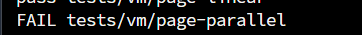
\includegraphics[width=\linewidth]{figures/result2.png}
    \end{figure}
    But if we try again, it would \textbf{pass}.
\end{frame}
%----------
\begin{frame}[fragile]{Results}
    \begin{figure}
        \centering
        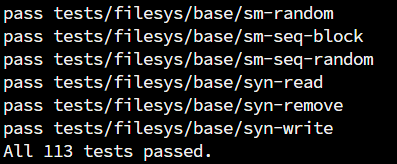
\includegraphics[width=0.6\linewidth]{figures/result.png}
        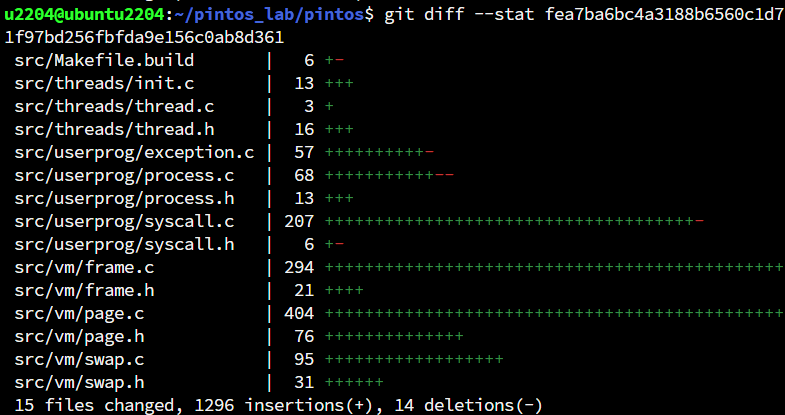
\includegraphics[width=0.8\linewidth]{figures/insert.png}
    \end{figure}
\end{frame}
%---
\begin{frame}[standout]
  \Large Thank you!\\
  Questions?
\end{frame}
\end{document}
